%&goedomteweten
\documentclass[presentatie.tex]{subfiles}

\begin{document}

\lang
{
    \section{\texorpdfstring{}{Good to know}}
}
{
    \section{\texorpdfstring{}{Goed om te weten}}%Goed om te weten}
}

\clearrecentlist

% \begin{frame}{Goed om te weten}
%     TODO Goed om te weten
% \end{frame}

\begin{saveblock}{code}
	\begin{highlightblock}[gobble=8,linewidth=0.5\textwidth,framexleftmargin=0.25em]
        Code
	\end{highlightblock}
\end{saveblock}

\begin{frame}
    {\lang,Installation,Installatie,}

    \href{https://vkuhlmann.com/latex/installation}{\nolinkurl{vkuhlmann.com/latex/installation}}

    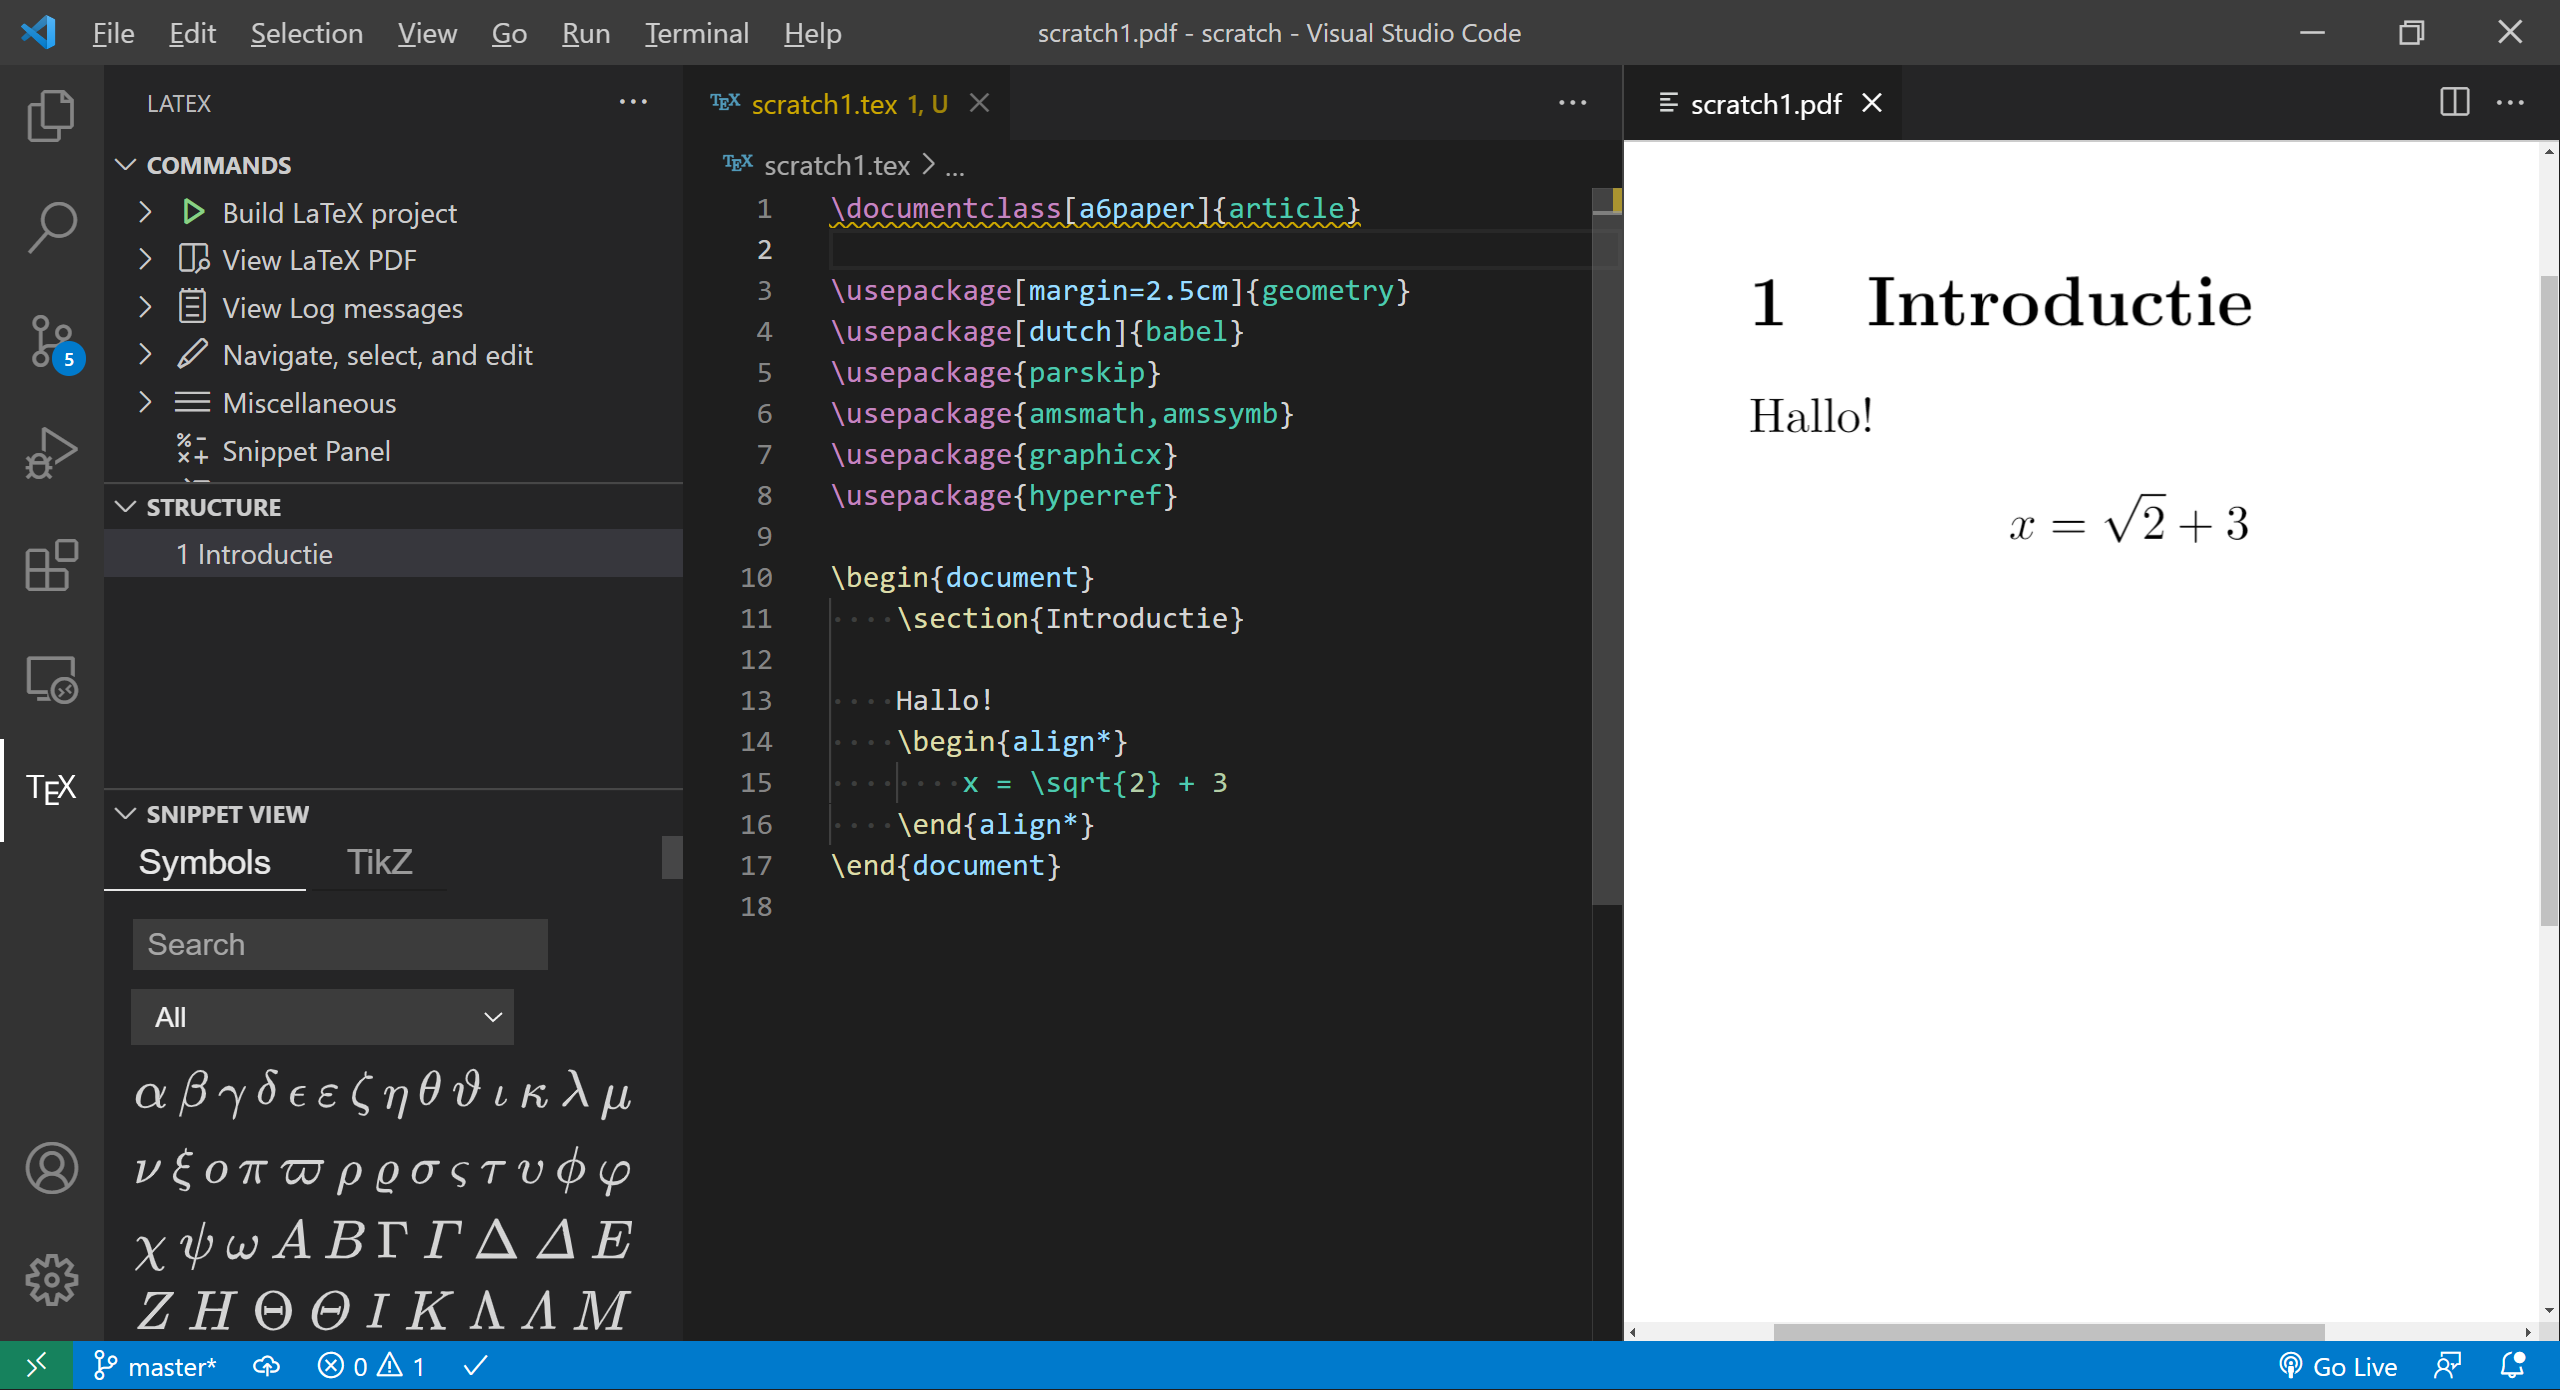
\includegraphics[width=\linewidth,height=0.8\textheight,keepaspectratio]{assets/Misc/VisualStudioCodeDemo.png}
\end{frame}

\begin{frame}
    \lang
    {On installed versions you might need to compile multiple times.}
    {Op installaties meermaals compileren.}
\end{frame}

\begin{frame}{The end}
	\begin{center}
		\LARGE \lang,Questions?,Vragen?,
	\end{center}

    \bigskip

    \begin{center}
        \lang{%
            Stuck? Mail us at\par
            \nolinkurl{texnicie@a-eskwadraat.nl}
        }{%
            Loop je vast? Mail ons op\par
            \url{texnicie@a-eskwadraat.nl}
        }
    \end{center}
\end{frame}

\end{document}
